\chapter{The Main Screen}
\section{Overview}
The Main Screen is the primary display screen. It is shown at power up, and is where Operation Mode (Hand or Automatic) is selected. It displays the Operator Message Centre which provides the Operator with current and relavent machine state information. There are also controls for \textit{Mode \textbf{Hand/Auto}}, \textit{Automatic \textbf{Cycle Start}} and \textit{Automatic \textbf{Cycle Stop}}, plus \textbf{\textit{Machine Full Stop}}. There is an information area for Saw details, and one for the current running cut program. Finally, there are screen navigation keys provided for Operator access to other machine functions.
\begin{figure}
	\centering
	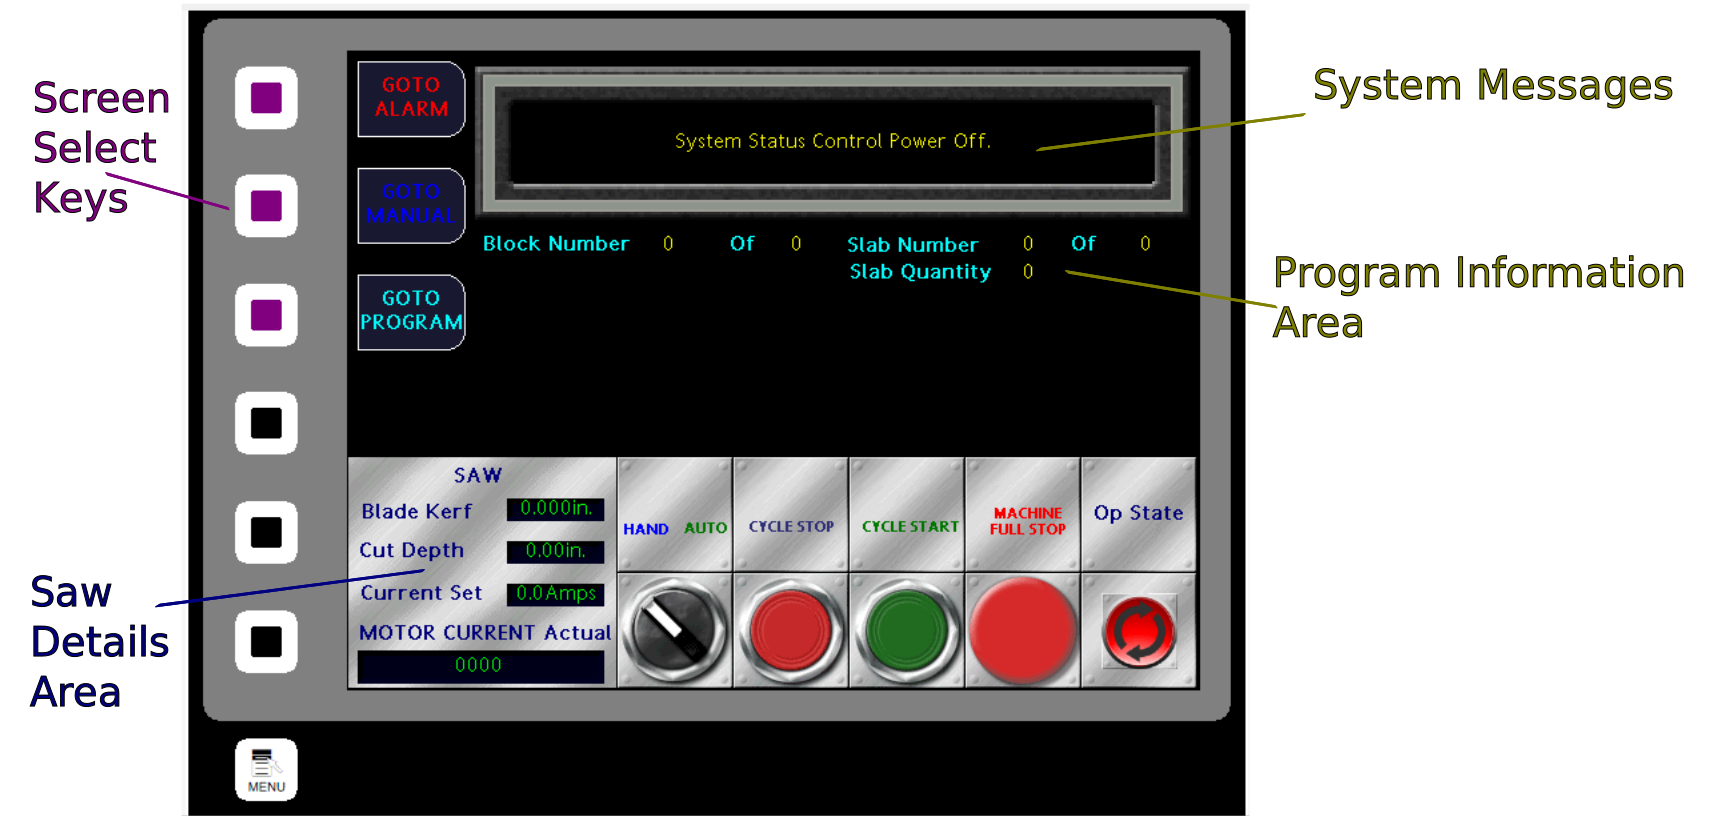
\includegraphics[width=0.5\linewidth]{screen-captures/main-screen}
	\caption{Main Screen}
	\label{fig:main-screen}
\end{figure}
\pagebreak
\section{Main Screen Details}
Main Screen Details are divided into the general categories.
\begin{list}{$\diamond$}{}
	\item \textbf{Screen Navigation}
	\item \textbf{Operator Message Centre}
	\item \textbf{Saw Information}
	\item \textbf{Program Details}
	\item \textbf{Operation Control}
\end{list}
\subsection{Screen Navigation}Is performed by using the programmable Function Keys (FKeys) located down the left hand side of the OI Terminal (refer to Figure 1.2). For the Main Screen there are three screens accessible using the labeled FKey's, \textbf{Alarms}, \textbf{Manual}, and \textbf{Program}.
\begin{figure}
		\centering
		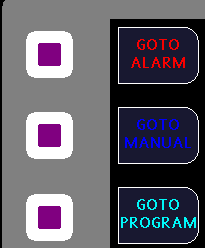
\includegraphics[width=.3\linewidth]{screen-captures/main-nav}
		\caption{Main Screen Navigation}
		\label{fig:main-nav}
\end{figure}
\begin{list}{$\diamond$}{}
	\item \textbf{GOTO ALARM} Navigate to Alarms Screen.
	\item \textbf{GOTO MANUAL} Navigate to Manual Screen.
	\item \textbf{GOTO PROGRAM} Navigate to Cut Program Screen.
\end{list}

\paragraph*{\textbf{\LARGE \textcolor{blue}{i}}}
The Menu Key located on the terminal at the lower left below the FKey's, will return the Operator to the Main Screen, from all other screens.\\
\begin{minipage}{4cm}
	\begin{picture}(20,70)
	
\includegraphics[width=.5\linewidth]{screen-captures/menu}
	\end{picture}
\end{minipage}\begin{minipage}[]{11cm}
\paragraph{\textbf{\LARGE \textcolor{blue}{i}}} The Menu Key is pictured as it looks on the Terminal.
\end{minipage}
\pagebreak
\subsection{Operator Message Centre}
Is the message display area located on the Main Screen near the Title. It is used to display information for the Operator during machine use. It doesn't display Alarms, that is done on the Alarms Screen, though it will indicate if an Alarm condition exists.
\begin{figure}
	\centering
	
\includegraphics[width=.5\linewidth]{screen-captures/message-centre}
	\caption{Main Screen Message Centre}
	\label{fig:main-msg-cntr}
\end{figure}
The \textit{Operator Message Centre} shown in Figure 1.3 will display information messages for the Operator. If more than one message is active the display will scroll through all messages continuously on a timed basis automatically. The Operator is not required to initiate any message change, or acknowledge a message, this display is merely for the Operator information.
\\
\\
\\
\\
\\
\\
\\
\\
\\
\\
\\
\\
\\
\\
\\
\pagebreak
\subsection{Saw Information}
Is an area where the Operator can see Saw information at a glance. \textbf{Saw Kerf}, \textbf{Cut Depth}, and \textbf{Current Set} are displayed along with the \textbf{Motor Current Actual}.
\\
\\
\begin{figure}
	\centering
	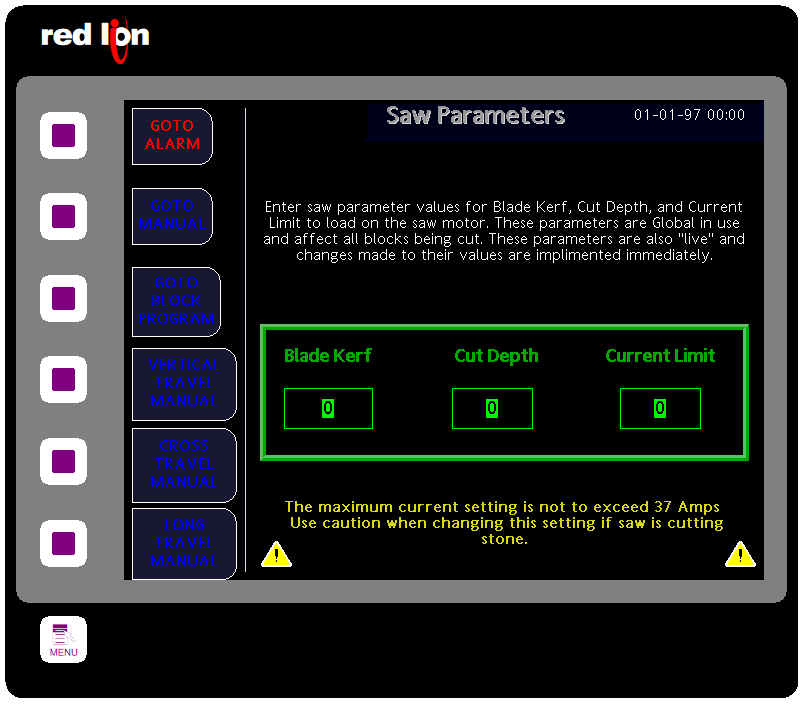
\includegraphics[width=.5\linewidth]{screen-captures/saw-info}
	\caption{Main Screen Saw Information}
	\label{fig:main-sawinfo}
\end{figure}
\textbf{\LARGE ( \textcolor{blue}{i} )} This information is display only, in order to make changes to the saw parameters \textit{Blade Kerf, Cut Depth, and Current Set} the operator must navigate to the Program Screen. Where they may be changed at any time and in any mode, even while running in automatic/manual or faulted. More details on those settings can be found in the chapter dealing with the Cut Program Screen.
\\
\\
\\
\\
\\
\\
\\
\\
\\
\\
\pagebreak
\subsection{Program Details} Display area will show the Operator details about the current block being cut as per the \textit{Cut Program} the Operator entered, while the Mode is automatic and the program is being executed. If the mode is automatic and the program execution is interrupted, or has completed, the display will show the last block details executed. If the Mode is Manual (Hand), and automatic operation has not been started/completed/interrupted, then it will display the first block of the cut program. Otherwise, the display will be the last block details from program execution, the same as if in Automatic mode. 
\\
\\
\textbf{\LARGE \textcolor{blue}{( i )}} The saw will keep track of where it is in the Cut Program execution cycle, even if cycle stop is pressed. Further details about how the Cut Program is executed, and what behaviour to expect from cycle interruption due to completion, alarms or Operator action can be found in the section(s) following.
\begin{figure}
	\centering
	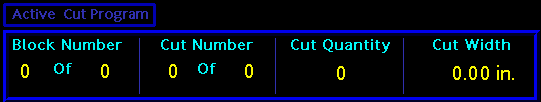
\includegraphics[width=.95\linewidth]{screen-captures/main-screen-prg-det}
	\caption{Main Screen Program Details}
	\label{fig:main-prg-det}
\end{figure}
The Program details (figure 1.5) will display information about the current Block being worked on, if running in Auto Cycle. If the cycle has been stopped, the details displayed will be about the current block being worked on, this is the same in both Hand and Auto Modes, as well as in the case of a faulted condition. This means that if the saw has finished cuts for a block entirely, the display will actually show details about the next block to work on since it is now the current block. If the cycle has completed without error, then the details of the last block programmed will be displayed, in either Hand or Auto Modes. If the program has not been run, and the Mode is either Hand or Auto (not in cycle) then the first block in the program will have it's details displayed. 
\\
\\
\\
\\
\pagebreak
\begin{figure}
	\centering
	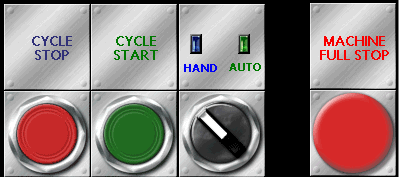
\includegraphics[width=.95\linewidth]{screen-captures/main-screen-opctl}
	\caption{Main Screen Operation Control}
	\label{fig:main-opctl}
\end{figure}
\subsection{Operation Control} Is provided by a group of Push Buttons and Selector Switches that allow the Operator to Select Modes (\textit{Hand/Auto)}), Start and Stop the Auto cycle (\textit{Cycle Start, Cycle Stop}) or execute a \textit{Machine Full Stop} command. 
\paragraph{\textbf{\LARGE \textcolor{blue}{( i )}}} The cut program may be restarted from any position, providing it was \textit{Cycle Stopped}. If the machine was stopped by pressing the \textit{Machine Cycle Stop} Button, the program will need to be re-entered as this is considered a faulted condition initiated by the Operator when machine safety is a concern. The same applies to any Fault generated by other emergent conditions that require the saw to be stopped mid-cycle. If the saw is stopped by pressing the \textit{Cycle Stop} Button, it may be placed into \textit{Hand} by the Operator if manual control is required. From a cycle stopped state, selecting \textit{Auto} and pressing \textit{Cycle Start} will restart the \textit{Cut Program} at the last known cut location and depth.
\paragraph{\textbf{{\LARGE \textcolor{red}{(!)}}}}Extreme Caution must be exercised when restarting the \textit{Cut Program} after a \textit{Cycle Stop}. If motion in the Long Travel Axis has been made after cycle stopping, there is a high probability that the saw will not return to the exact cut location due to mechanical tolerances in the axis. The saw will move the \textit{Vertical Axis} to the last programmed height when \textit{Cycle Stop} was pressed. Both of these conditions when combined, can lead to re-engaging a cut pass in a Block which is not perfectly in line with the original path the saw blade had established prior to stoppage. 
An example would be if the Long Axis was moved in the positive direction prior to a restart being issued, it would attempt to return to the last cut location from the home end of the machine. It accomplishes this type of move by traveling past the cut location back in the direction of home, then moving to the desired cut location. The repeatability of the saw position is not small enough to guarantee near perfect allignment of the blade with an existing cut. The vertical axis would then lower to the last cut height. If the saw blade is now near perfect in allignment with the existing cut location, the saw will finish the cut without incident due to misallignment. However, if the allignment is a blade width out in either direction, the potential for damage to product and possibly the equipment is greater.
\begin{figure}
	\centering
	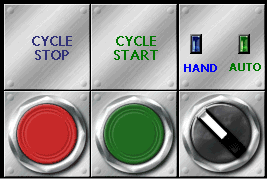
\includegraphics[width=.95\linewidth]{screen-captures/main-screen-mode-strt-stp}
	\caption{Main Screen Operation Control}
	\label{fig:main-mode-strt-stp}
\end{figure}
\subsubsection{Mode Set} Refer to Figure 1.7 shown above. The \textit{Hand/Auto} selector switch is provided for the Operator to be able to select \textit{Hand} or \textit{Auto} modes. Above both mode positions is an indicator light. As well as the switch position, the corresponding light will be on indicating which of the modes is selected. The blue light on will indicate that \textit{Hand} mode is selected. While the green light indicates \textit{Auto} mode is selected. When the selector is set to \textbf{\textit{Hand}}, the \textit{Blue} \textit{Hand} \textit{Indicator} will be on solid if no faults exist and flash if there is a fault, or if the machine needs homing of any axis. Selecting \textit{Hand} while in \textit{Auto} will change the mode to \textit{Hand}, even if a programmed cycle is running. When the \textit{Hand/Auto} selector switch is set to \textbf{\textit{Auto}}, the \textit{Green Auto Indicator} will flash if the saw is ready to run a cut program. In order to be ready to run a cut program in \textit{Auto} all of the saw axii must have been homed, no faults of any kind may exist, and a valid cut program must have been entered. When in \textit{Auto} mode, and once the \textbf{Cycle Start} pushbutton is pressed, the saw will begin \textit{Automatic} execution of the \textbf{Cut Program} the Operator entered and the \textbf{Auto} indicator will be on solid.
\subsubsection{Cycle Stop} When pressed while an \textit{Auto} cycle is executing a \textit{Cut Program}, will cycle stop the saw at completion of the currently executing step of the cycle. In practical terms what this means is that if the saw was moving to a new cut location, it would stop motion, and pause \textit{Auto} cycle, once that particular move was completed. This includes \textit{Cross Travel} motion, \textit{Vertical} motion, and \textit{Long Travel} motion. The saw will remain in \textit{Auto} mode after a \textbf{\textit{Cycle Stop}} has occurred.
\begin{figure}
	\centering
	
\includegraphics[width=.2\linewidth]{screen-captures/main-screen-mach-full-stop}
	\caption{Main Screen Machine Full Stop}
	\label{fig:main-mach-full-stop}
\end{figure}
\subsubsection{Machine Full Stop} Refer to Figure 1.8 above. \textbf{\textit{Machine Full Stop}} pushbutton is intended to be used in the event the Operator feels an immediate stop of automatic or manual motion is necessary. Unlike the \textbf{\textit{Cycle Stop}} pushbutton, pressing \textbf{\textit{Machine Full Stop}} will immediately stop all motion of the saw and exit \textit{Auto} mode. 
\paragraph*{\textbf{{\LARGE \textcolor{red}{!}}}}Unlike an Emergency Stop pushbutton, this is a programmed response to an Operator perceived hazard potential and \textbf{must not} be relied upon as a safety measure in any respect.
\paragraph*{\textbf{\LARGE \textcolor{blue}{i}}} A program that has been \textbf{\textit{Cycle Stop}}'d can be restarted from the stop location, even if the program has been changed within the limits of the program as it was running until then. What this means in practice is that if the Operator determined they need to correct an error in the cut program, in a part that hasn't been cut yet, they would be able to cycle stop the saw, correct the error, then \textbf{\textit{Cycle Start}} the program to continue.
\paragraph*{\textbf{{\LARGE \textcolor{red}{!}}}} If a program has been modified after a \textbf{\textit{Cycle Stop}} occurred, the restart of the cut program could generate and error if the data change exceeds the known saw limits. Refer to the chapter on \textbf{Cut Program} entry and details for further explanation.